%! Author = adnansiddiquei
%! Date = 04/06/2024

\section{Method}\label{sec:method}
Assuming that galaxy spectra and galaxy images can be viewed as different physical representations of the same underlying
object, reasonably, one can assume that there is enough mutual information within the two modalities to be able to effectively
embed them into a shared latent space.
As such, the objective of this piece of work was to reproduce the results of the original AstroCLIP paper~\citep{astroclip}
which implemented a multi-modal contrastive learning approach to embed galaxy spectra and galaxy images into a shared embedding
space.
This was done using 2 pretrained convolutional spectrum and image embedders, and then fine-tuning the model using contrastive
learning under the InfoNCE loss~\citep{oord2019}, as per Equation~\eqref{eq:infonce}, to learn the low-dimensional
embedding space for the two modalities

\begin{equation}
\label{eq:infonce}
    \mathcal{L}(\mathbf{X}, \mathbf{Y}) = - \frac{1}{K} \sum_{i=1}^K \log \frac{\exp(S_C(\mathbf{x}_i, \mathbf{y}_i) / \tau)}{\sum_{j}^K \exp(S_C(\mathbf{x}_i, \mathbf{y}_j) / \tau)}.
\end{equation}
where $\mathbf{X}$ and $\mathbf{Y}$ is an embedded batch of sets of galaxy spectra and images, $K$ is the size of the
batch, $S_C$ is the cosine similarity function, and $\tau$ is a smoothing parameter (often called the temperature).
Indices $i$ correspond to positive pairs (embedded image-spectra pairs which correspond to the same galaxy) and $j$ corresponds
to negative pairs (embedded image-spectra pairs which correspond to different galaxies).
Formerly, $S_C$ defined in Equation~\eqref{eq:cosine-similarity}

\begin{equation}
\label{eq:cosine-similarity}
    S_C(\mathbf{x}_i, \mathbf{y}_j) = \frac{(\mathbf{x}_i)^{T} \mathbf{y}_j}{ ||\mathbf{x}_i||_{2} \hspace{0.2em} ||\mathbf{y}_j||_{2}}
    = \cos(\theta_{i,j})
\end{equation}

is the normalised dot product between any two embeddings, where $\theta_{i,j}$ is the angle between the two embeddings.
The similarity measure $S_C$ is bounded in the range [-1, 1], and by construction, for any two embeddings which refer to
the same galaxy then $S_C(\mathbf{x}_i, \mathbf{y}_i)) = 1$ given that $\theta_{i,i} = 0 \hspace{0.25em} \forall i$.

\subsection{Data}\label{subsec:data}
We use the dataset as provided exactly by~\cite{astroclip}, with minor adjustments.
The dataset contains 197,976 galaxy spectra and image pairs, along with their redshift measurements.
The galaxy spectra were taken from the Dark Energy Spectroscopic Instrument (DESI) Early Data Release~\citep{desiearly2023}
and the galaxy images were taken from the DESI Legacy Survey~\citep{desilegacy2018}.
We summarise the key pre-processing steps relating to the data below.

\subsubsection{DESI Legacy Survey Images}\label{subsubsec:images}
The galaxy image dataset was curated by~\cite{stein2022} from the DESI Legacy Survey Data Release 9\footnote{https://www.legacysurvey.org/dr9/description/},
we refer the reader to~\cite{stein2022, astroclip} for a more comprehensive overview of the dataset and its curation, but the
key points are summarised here.
These images were taken by 3 different telescopes, with each telescope focusing on a different combination of sky area
and wavelength range, creating a survey of the sky with a sky coverage of 14,000 $deg^{2}$, at a pixel resolution of 0.262 arcseconds,
across the g (green: $4770 \si{\angstrom}$), r (red: $6231 \si{\angstrom}$), and z (infrared: $9134 \si{\angstrom}$) wavelength
bands\footnote{https://skyserver.sdss.org/dr1/en/proj/advanced/color/sdssfilters.asp}.
The Tractor\footnote{https://github.com/dstndstn/tractor} is used to probabilistically identify and infer properties such
as morphological classification of sources within the survey.
This creates a Tractor catalogue of each identified source, and a sweep catalogue is a subset of this information.
~\cite{stein2022} then filter the dataset as follows: they drop any source that were identified as a star in the sweep catalogues
(Tractor identified a best-fit morphological model of point-spread function, which indicates star); and drop any sources
with a z-band magnitude ($mag_{z}$) larger than 20.
Each remaining source is extracted through a 256x256 pixel cut-out centred on the source, in each of the (g, r, z) bands,
yielding a total of 76,446,849 images.
~\cite{astroclip} cross-match this dataset for their corresponding spectra from the DESI Early Data Release~\citep{desiearly2023}
using the targetIDs associated with the sources, to yield a final dataset of 197,976 galaxy spectra and image pairs.

We perform a variety of augmentations on the images including: a random horizontal and vertical shift; random rotation;
random horizontal and vertical flips as well as adding Gaussian noise.
The 256x256 pixel images all cover more sky than the source being analysed, so we follow~\cite{stein2022} in center
cropping the images to the central 96x96 pixels, adverse to the 144x144 cut-out performed by~\cite{astroclip}.
The choice of the 96x96 cut-out as opposed to a 144x144 cut-out is primarily due to the pre-training of our image embedder
as explained in Section~\eqref{subsubsec:image-embedder}.
The images are then standardised, ensuring that each channel (g, r, z) of each image had a mean
of 0 and a standard deviation of 1.
The Gaussian noise $\mathcal{G}(0, 0.03)$ was added on top of this standardised data such that each channel was noised
proportionately.


\subsubsection{DESI Early Data Release Spectra}\label{subsubsec:spectra}
The spectra were extracted from the DESI Early Data Release~\citep{desiearly2023} and only those that were successfully
cross-matched with the galaxy images were kept.
The spectra ranged the wavelength range of $[3600 \si{\angstrom}, 9824 \si{\angstrom}]$, with a resolution of 7781 pixels per spectrum.
As with the image data, the spectra were also standardised individually, to mean 0 and standard deviation 1, and then
noise $(\epsilon_{sp}(\lambda))$ was added in the form of scaled Gaussian noise as given in Equation~\eqref{eq:spectrum-noise}.

\begin{equation}
\label{eq:spectrum-noise}
    \epsilon_{sp}(\lambda) = \gamma \cdot \sigma_{sp}(\lambda) \cdot \mathcal{G}(0, 1)
\end{equation}
where $\epsilon_{sp}(\lambda)$ is the noise added to the spectrum at wavelength $\lambda$, $\gamma$ is a scaling factor
which is the same for all wavelengths, $\sigma_{sp}(\lambda)$ is the standard deviation of the spectrum at wavelength $\lambda$,
and $\mathcal{G}(0, 1)$ is a standard Gaussian random variable.
$\sigma_{sp}(\lambda)$ was computed for the training set such that $\sigma_{sp}(i)$ $(i \in [0, 7781])$ gave the standard
deviation of all spectra measurements at the $i^{th}$ pixel.
This meant that the noise added to the spectra at any given wavelength was proportional to the variance of the spectra
the given wavelength, which complemented the fact that some wavelengths naturally had more variance than others.
Finally, $\gamma$ was set to 0.3.

\subsubsection{Redshift measurements}\label{subsubsec:redshift}
The redshift measurements utilised were the catalog-reported measurements and were compiled and provided directly with the
dataset by~\cite{astroclip}.

\subsubsection{Further Pre-processing}\label{subsubsec:pre-processing}
The data was pre-processed further to remove outliers and ensure data was sensible to improve training dynamics.
We dropped any galaxies with a redshift outside the range $[0, 0.8]$ and also dropped any galaxies which had every element
in their spectra equal to 0 (given that they were clearly erroneous).
This resulted in removing a further 380 samples from the dataset, leaving a total of 197,596 galaxy spectra and image pairs.
Our redshift range of $[0, 0.8]$ was larger than the range of $[0, 0.6]$ used by~\cite{astroclip} in their final results.

\subsection{AstroCLIP Implementation}\label{subsec:astroclip-implementation}
Our AstroCLIP model was implemented using a pretrained 2D convolutional image embedder courtesy of~\cite{stein2021}
and a pretrained 1D spectrum embedder courtesy of~\cite{liang2023}.
These were placed into our unified AstroCLIP model and then fine-tuned (with all the weights set as trainable) using
contrastive learning under the InfoNCE loss as per Equation~\eqref{eq:infonce}, to learn the shared low-dimensional
embedding space.
Embeddings were projected into a variety of dimensions: (8, 16, 32, 64, 128, 256, 512) to explore the effect of the
dimensionality of the embedding space on the performance of the model, with~\cite{astroclip} using a 512 dimensional
embedding for their final results.
Below we give a brief overview of the pretraining strategies for the image and spectrum embedders, but for a
comprehensive report we refer the reader to the original papers.

\subsubsection{Image Embedder}\label{subsubsec:image-embedder}
\cite{stein2021} trained a galaxy image embedder using a self-supervised method for the purposes of image based similarity search.
The image embedder was trained via the MoCo v2 framework~\citep{moco2020, mocov22020} on a sample of 42 million galaxies
from the DESI Legacy Survey Data Release 9~\citep{desilegacy2018}.
The encoder architecture used was a ResNet-50 architecture.
The images underwent a variety of augmentations (galactic extinction, random rotation, blurring, noising) before
being cropped to the central 96x96 pixels.
The loss function used was the same InfoNCE loss we used in our AstroCLIP model as given in Equation~\eqref{eq:infonce},
and the similarity measure used was also the cosine similarity function as given in Equation~\eqref{eq:cosine-similarity}.
Their model yielded very promising results, and we refer the reader to the original paper for a thorough discussion
on the trained model.
The final fully-connected layers of this model contained 3 layers with 2048, 2048 and 128 units respectively.
The final 128 unit layer was adjusted as required to produce the output dimensionality we desired, but otherwise all
weights and biases were initiated as per the pretrained model.
This yielded between 27.7M and 28.8M trainable parameters depending on the output dimensionality of the model.

\cite{astroclip} pre-train a vision transformer model for their image embedder, we refer the reader to the original paper
for a more detailed discussion on the architecture and pre-training strategy for this.

\subsubsection{Spectrum Embedder}\label{subsubsec:spectrum-embedder}
\cite{liang2023} trained a galaxy spectrum autoencoder using galaxy spectra from the DESI Early Data Release~\citep{desiearly2023},
focusing primarily on the Bright Galaxy Survey (BGS) (for precise details on the spectral dataset used, see the original paper).
The autoencoder architecture, named SPENDER, was proposed by~\cite{melchior2022} and encoded the spectra into a 6-dimensional
embedding space.
For our AstroCLIP model, we used the encoder part of the SPENDER model which consisted of a series of 1D convolutional layers
followed by a series of fully-connected layers to bring the dimensionality down to 6.
We reduced the fully-connected layers to 3 layers with 256, $D_{-1}$ and $D_{out}$ units respectively, for any desired
output dimensionality $D_{out}$.
The first 2 fully-connected layers in the pre-trained SPENDER encoder originally had a dimensionality of 256 and 128 units
and as such, for $D_{out} \in [8, 16, 32, 64, 128]$, we retained $D_{-1}=128$ and so the weights and biases of the
first 2 fully-connected layer were retained with the output layer being initialised from a Gaussian distribution.
For $D_{out} \in [256, 512]$, $D_{-1}$ was set to 256 and the entire fully-connected part of the model was retrained
from Gaussian initialisation.
The convolutional layers were initialised from the pre-trained weights of the SPENDER model.
This yielded between 3.1M to 3.3M trainable parameters, depending on the output dimensionality of the model.

\cite{astroclip} once again use a transformer architecture for their spectrum encoder, and we refer the reader to the original
paper for a more detailed discussion on the architecture and pre-training strategy for this.

\subsection{Training}\label{subsec:training}
\begin{figure}[t]
    \centering
    \makebox[\textwidth]{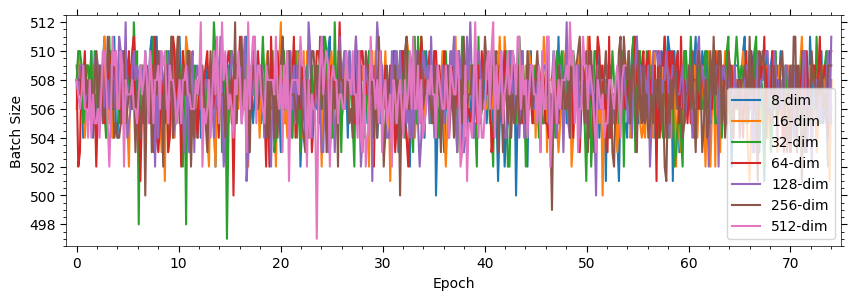
\includegraphics[width=0.9\textwidth]{figures/train_batch_size}}
    \caption{The batch size for each batch after the pre-processing steps were applied to the batch on the fly.
    Each line represents the batch size throughout the training of AstroCLIP models with everything identical except the
    embedding dimensionality.
    The individual lines are not meant to be discernable from one another, but rather this figure should show the general trend.}
    \label{fig:train_batch_size}
\end{figure}

\begin{figure}[t]
\centering
\begin{subfigure}{1\textwidth}
  \centering
  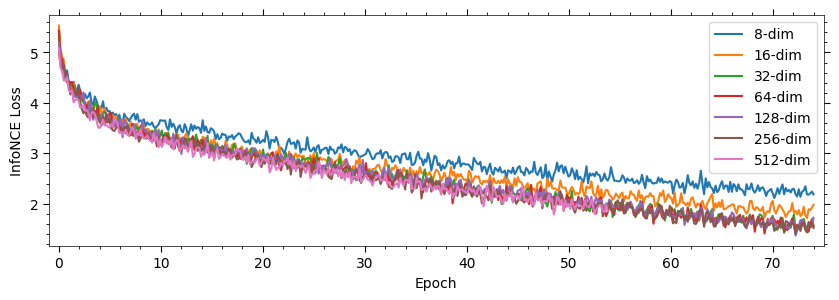
\includegraphics[width=0.9\linewidth]{figures/train_loss}
  \caption{Training loss.}
  \label{fig:train_loss}
\end{subfigure}%
\hfill
\begin{subfigure}{1\textwidth}
  \centering
  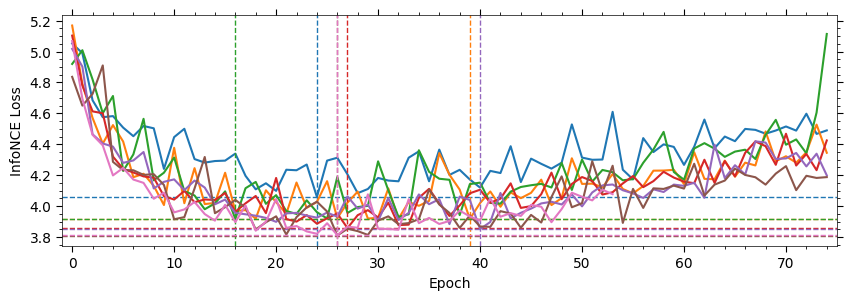
\includegraphics[width=0.9\linewidth]{figures/val_loss}
  \caption{Validation loss.
  The vertical lines correspond to the epoch at which the lowest validation loss was achieved and the horizontal
  line corresponds to the loss value at that epoch.
  The (embedding dimensionality, lowest validation loss, epoch) values are as follows: (8, 4.06, 24); (16, 3.92, 39);
  (32, 3.92, 16); (64, 3.86, 27); (128, 3.85, 40); (256, 3.81, 26); (512, 3.81, 26).}
  \label{fig:val_loss}
\end{subfigure}
\caption{Train and validation loss for AstroCLIP models with varying embedding dimensionality.
The legend on Figure~\eqref{fig:train_loss} applies to both plots.}
\label{fig:train_val_loss}
\end{figure}

Our AstroCLIP model unifies these two embedders into a single model, and then fine-tunes the embeddings using the InfoNCE loss
(Equation~\eqref{eq:infonce}).
The embedding dimensionality was varied through the range $[8, 16, 32, 64, 128, 256, 512]$ and each model was trained for
75 epochs.
Through some exploratory analysis, we fixed a few hyperparameters: batch size of 512; learning rate of $5e^{-4}$; a weight
decay of $1e^{-4}$; and a temperature parameter in the InfoNCE loss of 0.07; and only varied the embedding dimensionality.
One small aspect of note is that the batch size was not consistent throughout training, the pre-processing mentioned in
Section~\eqref{subsubsec:pre-processing} was performed on the fly on each batch of data as and when randomly sampled by
the DataLoader during training.
This meant that there were small fluctuations in the batch size, and for completeness we show the batch size for each batch
throughout the training of the AstroCLIP models in Figure~\eqref{fig:train_batch_size}.
As can be seen on the figure, the batch size fluctuates very little and generally remains between 502 and 510.
This fluctuating batch size was intentionally left in the training process as it's effects were negligible and would likely
only have a positive effect through the stochasticity it introduces.
The number of epochs required to reach the lowest validation loss, and the corresponding loss is detailed in Figure~\eqref{fig:val_loss}.
Whilst there is a clear pattern in the training loss where the more flexible model appears to be able to achieve the
lowest loss, the same was not true for the validation loss with no clear pattern emerging.
However, it is important to note that a thorough sweep of hyperparameters was not performed, and so it is possible that
a different set of hyperparameters (such as stronger regularisation on the more flexible models, to prevent over-fitting)
could have yielded different results (lower validation loss for the more flexible models).
The models with the lowest validation loss for each embedding dimensionality were selected for evaluation in Section~\eqref{sec:results}.
